% "{'classe':('PSI'),'chapitre':'slci_ap','type':('td'),'titre':'Train d’atterrissage d\\'hélicoptère', 'source':'Banque PT - SIA 2014','comp':('C1-02','C2-04'),'corrige':True}"
%\setchapterimage{bandeau}
\chapter*{TD \arabic{cptTD} \\ 
Avance de Phase -- Train d’atterrissage d'hélicoptère \ifnormal $\star$ \else \fi \ifdifficile $\star\star$ \else \fi \iftdifficile $\star\star\star$ \else \fi  -- 
\ifprof Corrigé \else Sujet \fi}
\addcontentsline{toc}{section}{TD \arabic{cptTD} :
Avance de Phase -- Train d’atterrissage d'hélicoptère \ifnormal $\star$ \else \fi \ifdifficile $\star\star$ \else \fi \iftdifficile $\star\star\star$ \else \fi  -- 
\ifprof Corrigé \else Sujet \fi}

\iflivret \stepcounter{cptTD} \else
\ifprof  \stepcounter{cptTD} \else \fi
\fi

\setcounter{question}{0}
\marginnote{Banque PT -- SIA 2014.}
\marginnote[1cm]{
\UPSTIcompetence[2]{C1-02}
\UPSTIcompetence[2]{C2-04}}

\begin{marginfigure} [4cm]
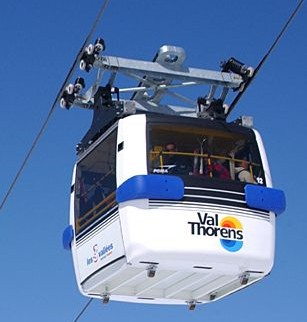
\includegraphics[width=\linewidth]{fig_00}
\end{marginfigure}



\section*{Mise en situation}
\ifprof
\else
Lors d’atterrissages d'hélicoptères à grande, les oscillations induites par l'impact au sol du train
d'atterrissage principal génèrent des contraintes mécaniques importantes à la liaison du pylône de queue avec
la cabine. Les oscillations du pylône de queue de l’appareil ne sont pas négligeables.
Lors de ces atterrissages, les vitesses verticales minimales sont de l’ordre de \SI{2}{m.s^{-1}} mais peuvent atteindre des valeurs plus importantes lors d’appontage sur un bateau à cause des mouvements du bateau dus à la houle.
La résistance aux crashs correspond à la possibilité de garder opérationnel un appareil qui aurait atterri avec
une vitesse d'impact pouvant atteindre \SI{4}{m.s^{-1}}.
%\begin{center}
%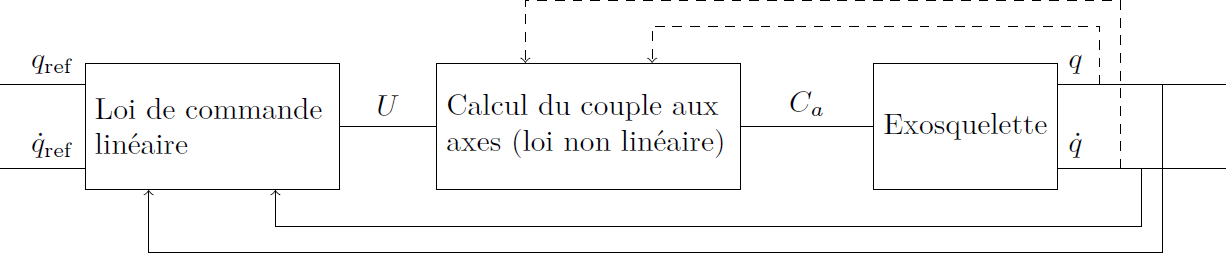
\includegraphics[width=.8\linewidth]{fig_07}
%%%\textit{}
%\end{center}
\fi
\begin{obj}
Pour une vitesse d'impact de \SI{4}{m.s^{-1}} l'accélération de la queue doit rester inférieure à \SI{3}{rad.s^{-2}}.
\end{obj}

\ifprof
\else

On donne une modélisation cinématique du train principal. 
\begin{center}
\begin{minipage}[c]{.48\linewidth}
\begin{center}
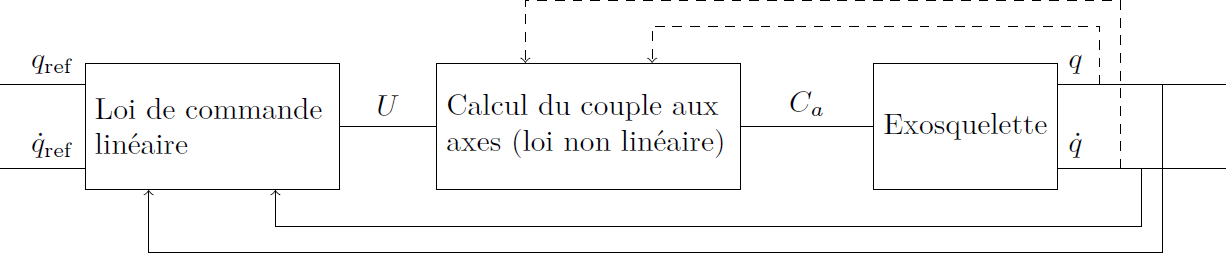
\includegraphics[width=\linewidth]{fig_07}
%%\textit{}
\end{center}
\end{minipage} \hfill
\begin{minipage}[c]{.48\linewidth}
\begin{center}
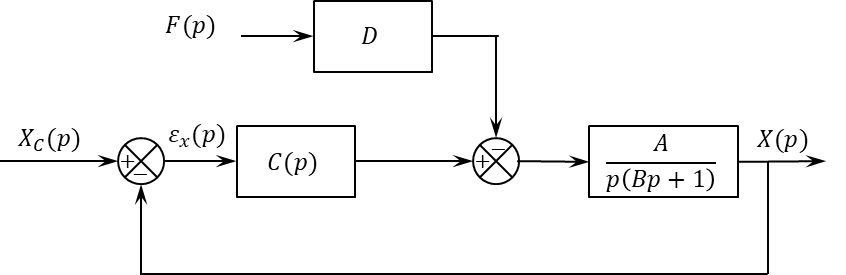
\includegraphics[width=\linewidth]{fig_08}
%%\textit{}
\end{center}
\end{minipage} \end{center}
La vitesse d'impact lors de l'atterrissage de l'hélicoptère correspond alors à la vitesse de la tige 5 de l'amportisseur par rapport au cylindre 4. Cette vitesse est notée $Z^*$. On se propose d'étudier la stabilité vis-à-vis de la seule consigne  $\dot{Z}_c^*(p)$. On adoptera pour le réglage de la correction le schéma suivant.

%\begin{center}
%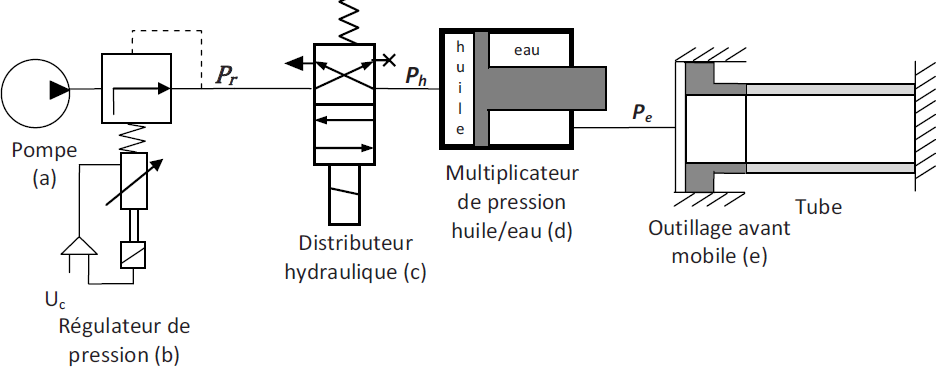
\includegraphics[width=\linewidth]{fig_01}
%%\textit{}
%\end{center}


\footnotesize
\begin{center}
\begin{tikzpicture}[scale=0.85, every node/.style={scale=0.85}]

\sbEntree{E}

\sbComp{c1}{E}
    \sbRelier[$\dot{Z}^*_C(p)$]{E}{c1}

\sbBloc{b1}{$C(p)$}{c1}
    \sbRelier{c1}{b1}

\sbBloc{b2}{$H_S(p)$}{b1}
    \sbRelier{b1}{b2}
    
\sbComp[6]{c2}{b2}
  \sbRelier[$F_{\text{éq}}(p)$]{b2}{c2}

\sbBloc{b3}{$H_Z(p)$}{c2}
    \sbRelier{c2}{b3}

\sbBloc{b4}{$\dfrac{1}{p}$}{b3}
    \sbRelier{b3}{b4}
%\sbBloc{b2}{$H_2(p)$}{c2}
  %  \sbRelier{c2}{b2}
    

\sbSortie[4]{S}{b4}
    \sbRelier{b4}{S}
    \sbNomLien[0.8]{S}{$\dot{Z}^*(p)$}

\sbDecaleNoeudy[4]{b4}{n1} 
\sbDecaleNoeudx[-2]{n1}{n2} 

\sbBlocr{r}{$\lambda_a$}{n2} 
\sbRelieryx{b4-S}{r}
\sbRelierxy{r}{c2}

\sbDecaleNoeudx[4]{b4}{n3} 
\sbDecaleNoeudy[-.4]{n3}{n4} 
\sbRenvoi[6]{n4}{c1}{}

%\draw [latex-] (c2) --++ (0,1) node[left] {$\text{Pert}(p)$};

\end{tikzpicture}
\end{center}
\normalsize


On note dans ce schéma :
\begin{itemize}
\item $\dot{Z}^*(p)$ la transformée de $\dot{z}^*(t)=\dot{z}(t)+V_0$  avec $V_0$ la vitesse d'impact et $\dot{z}(t)$ la vitesse absolue de la cabine par rapport au sol;% (voir figure 8 annexe 5).
\item $F_{\text{éq}}(p)$  l'effort équivalent ramené au déplacement de la cabine et fourni par la partie active de l'amortisseur;% (voir partie D1).
\item $\lambda_a$ le coefficient d'amortissement passif équivalent ramené au déplacement de la cabine;
\item $H_S(p)=\dfrac{K_S}{1+T_Sp}$ la fonction de transfert de la partie active de l'amortisseur. %Indépendamment de la partie précédente, 
On prendra : $K_S = \SI{12e4}{N.A^{-1}}$ et $T_S = \SI{5e-3}{s}$;
\item $H_Z(p)=\dfrac{K_Z p^2}{1+\dfrac{2\xi_Z}{\omega_Z}p+\dfrac{p^2}{\omega_Z^2}}$ la fonction de transfert traduisant le comportement dynamique du train.
\item $C(p)$ la fonction de transfert du correcteur dont le réglage fait l'objet de cette partie.
\end{itemize}
%$\dot{Z}_c^*(p)$  est la transformée de la consigne  $\dot{z}_c^*(t)$. On donne ci-dessous l'allure de la consigne en vitesse avec une accélération de $\SI{12}{m.s^{-2}}$ et une vitesse maximale de $\SI{4}{m.s^{-1}}$. 
%
%
%\begin{center}
%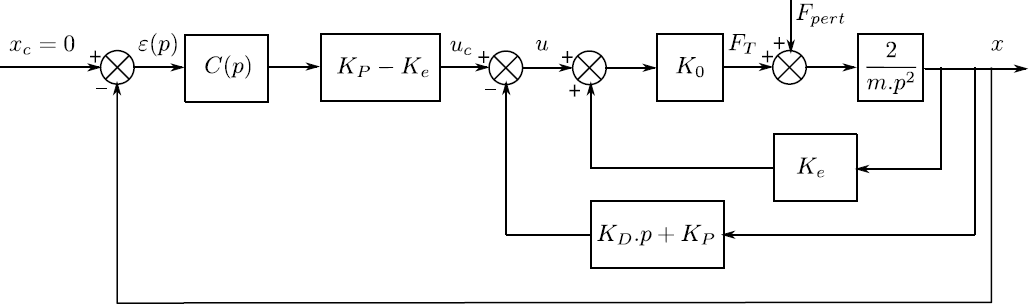
\includegraphics[width=.5\linewidth]{fig_02}
%%\textit{}
%\end{center}
\fi


\subsection*{Fonction de transfert en boucle ouverte non corrigée}
\begin{obj}
II s'agit dans un premier temps d'analyser la forme de la fonction de transfert en boucle ouverte non corrigée de la chaîne de commande semi-active.
\end{obj}

\question{Déterminer littéralement et sous forme canonique la fonction de transfert  $H_F(p)=\dfrac{\dot{Z}^*(p)}{F_{\text{éq}}(p)}$.}
\ifprof
\begin{corrige}~\\
$H_F(p) = \dfrac{H_Z(p)\dfrac{1}{p}}{1+\lambda_a H_Z(p)\dfrac{1}{p}}= \dfrac{\dfrac{K_Z p^2}{1+\dfrac{2\xi_Z}{\omega_Z}p+\dfrac{p^2}{\omega_Z^2}}\dfrac{1}{p}}{1+\lambda_a \dfrac{K_Z p^2}{1+\dfrac{2\xi_Z}{\omega_Z}p+\dfrac{p^2}{\omega_Z^2}}\dfrac{1}{p}}$
$= \dfrac{K_Z p^2}{p\left( 1+\dfrac{2\xi_Z}{\omega_Z}p+\dfrac{p^2}{\omega_Z^2} \right)+\lambda_a K_Z p^2}$

$= \dfrac{K_Z p}{ 1+\left(\dfrac{2\xi_Z}{\omega_Z}+\lambda_a K_Z\right)p+\dfrac{p^2}{\omega_Z^2} }$.
\end{corrige}
\else
\fi

\question{Déterminer littéralement la fonction de transfert en boucle ouverte non corrigée $H_{\text{BONC}}(p)$.}
\ifprof
\begin{corrige}
$H_{\text{BONC}}(p) = \dfrac{K_Z p}{ 1+\left(\dfrac{2\xi_Z}{\omega_Z}+\lambda_a K_Z\right)p+\dfrac{p^2}{\omega_Z^2} } \cdot \dfrac{K_S}{1+T_Sp} $.
\end{corrige}
\else
\fi


\ifprof
\else

\begin{marginfigure}
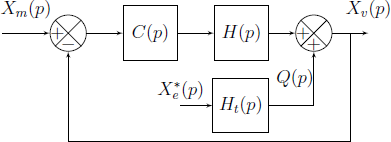
\includegraphics[width=\linewidth]{fig_03}
%\textit{}
\end{marginfigure}
\fi

On donne le diagramme de Bode de $H_F(p)$.

\question{Justifier la forme de ce diagramme en traçant les asymptotes et en indiquant comment retrouver sur le tracé les valeurs de $K_z$ et $\omega_z$. Tracer en rouge les diagrammes de la fonction $H_{\text{BONC}}(p)$. On prendra pour cela $20\log K_S \simeq \SI{100}{dB}$.}
\ifprof
\begin{corrige}
$H_F$ est un second ordre dérivé de coefficient d'amortissement $\xi_{F}$ et de pulsation propore $\omega_{Z}$. Ne pouvant pas calculer $\xi_{F}$, l'allure du diagrame de Bode suggère que $\xi_{F}<1$ car il y a une seule rupture de pente à $\omega_Z= \SI{5,5}{rad.s^{-1}}$.

Pour $\omega<\omega_Z$< l'asymptote du second ordre à un gain de $\SI{0}{dB}$. Seul le dérivateur est influent. En conséquence, pour $\omega =\SI{1}{rad.s^{-1}}$, on a donc $\left| K_Z p\right|_{\text{dB}}=20\log K_Z=-106$. On a donc $K_Z=5\times 10^{-6}$. 

\begin{center}
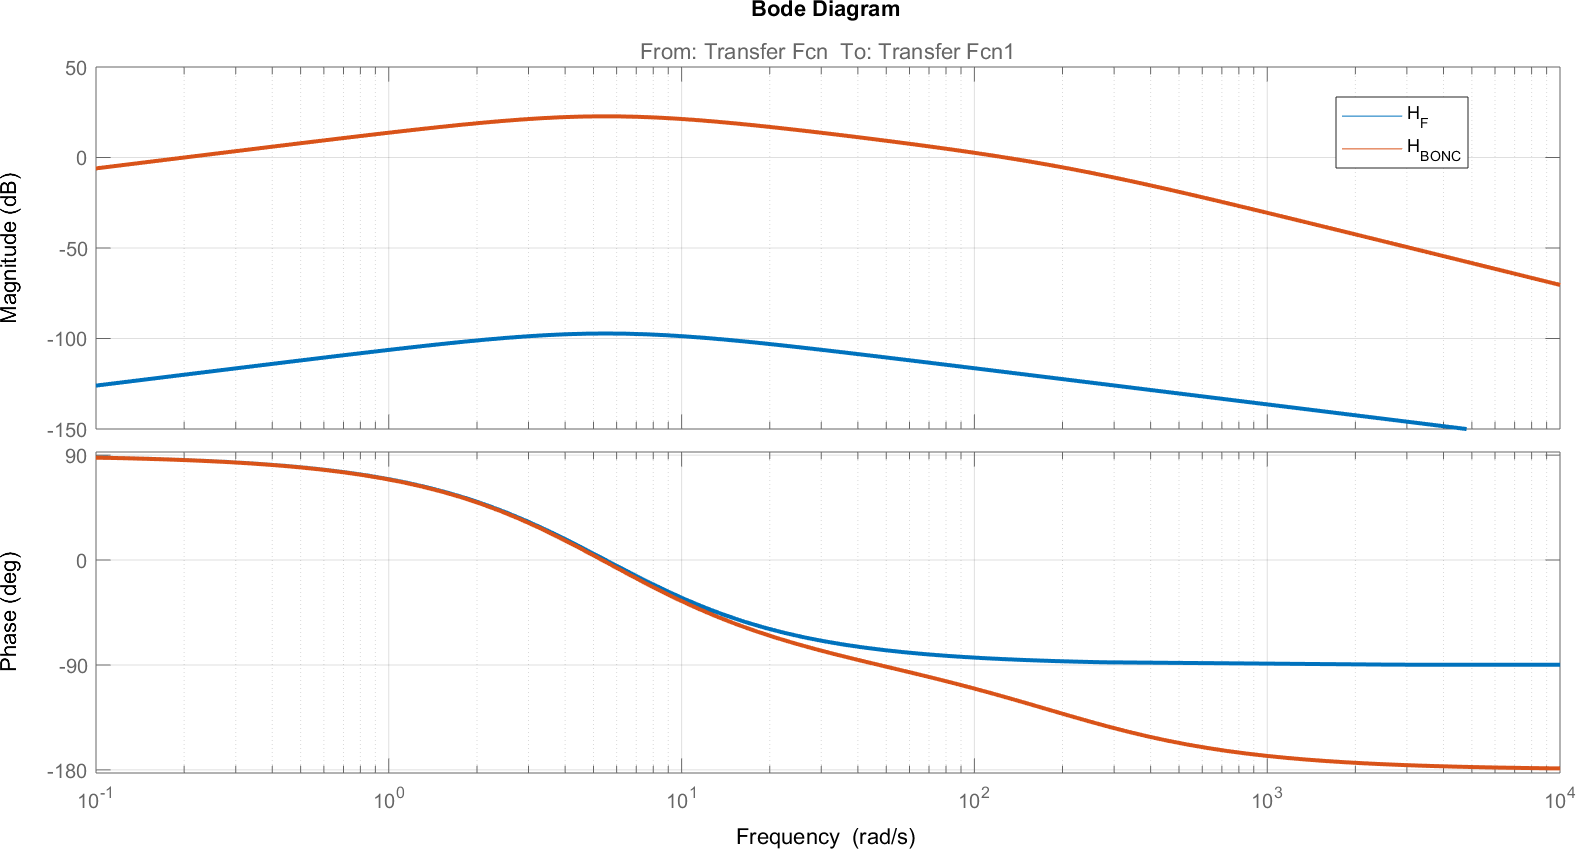
\includegraphics[width=\linewidth]{BODE_NC.png}
%\textit{}
\end{center}
\end{corrige}
\else
\fi

\subsection*{Choix et réglage de la correction}
\begin{obj}
II s'agit à présent de définir la structure du correcteur et de proposer un réglage permettant de satisfaire les critères du cahier des charges.
\end{obj}
\ifprof
\else
Afin de satisfaire les exigences, une étude complémentaire non abordée dans ce sujet montre que la boucle d'asservissement doit posséder les performances suivantes :
\begin{itemize}
\item erreur statique nulle;
\item pulsation de coupure à \SI{0}{dB} et $\omega_{\SI{0}{dB}}= \SI{6}{rad.s^{-1}}$;
\item marge de phase $M\varphi = 45\degres$;
\item marge de gain $MG > \SI{6}{dB}$.
\end{itemize}
\fi

\question{Quelle doit être la classe minimale du correcteur afin de garantir le critère de précision ?}
\ifprof
\begin{corrige}
Pour que l'erreur statique soit nulle, il faut que la classe de la FTBO soit de 1. La classe de la FTBO non corrigée étant de <<$-1$>>, il faut donc que le correcteur soit de classe 2 pour que le critère de précision soit garanti.
\end{corrige}
\else
\fi

\ifprof
\else
On choisit dans un premier temps un correcteur de la forme $C(p)=\dfrac{K_p}{p^2}$. On donne les diagrammes de Bode de la fonction de transfert en boucle ouverte du système ainsi corrigé pour $K_p =1$. 

\begin{marginfigure}
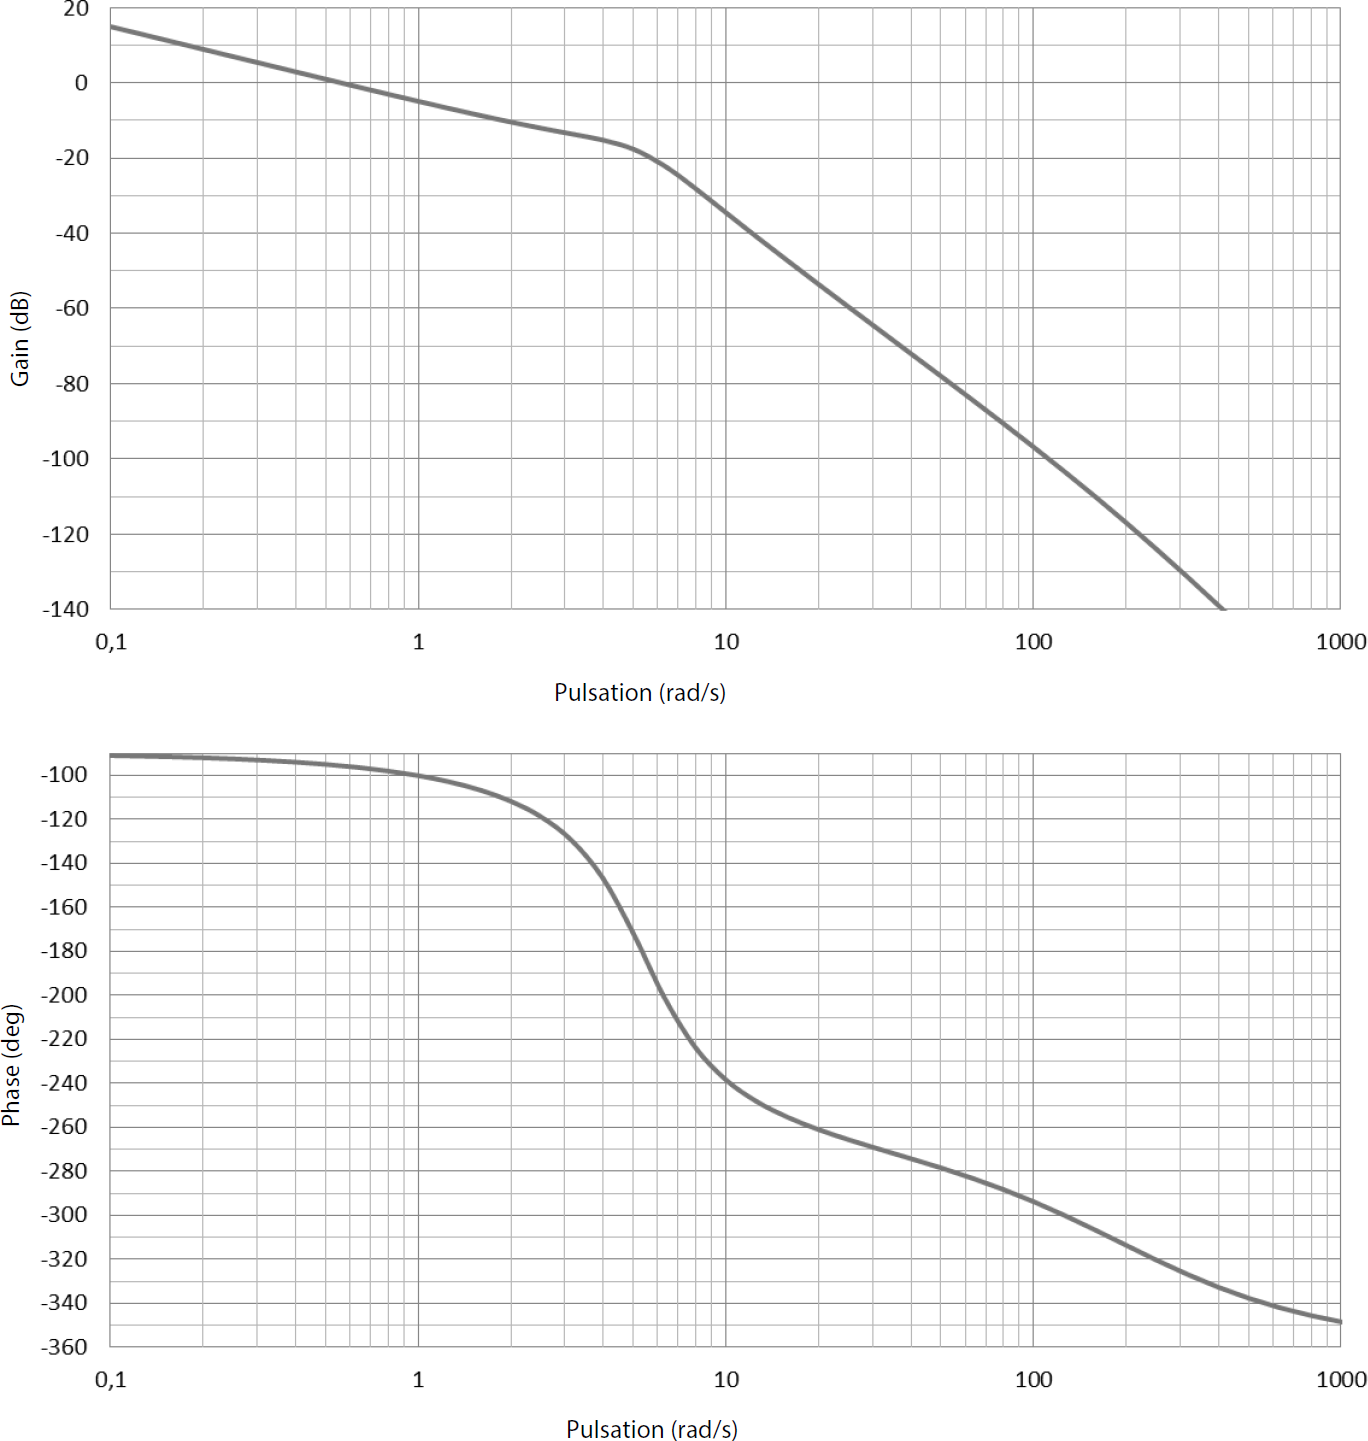
\includegraphics[width=\linewidth]{fig_04}
%\textit{}
\end{marginfigure}

\fi

\question{Évaluer les marges de stabilité pour ce réglage. Déterminer la valeur de $K_p$ garantissant le critère de pulsation de coupure à \SI{0}{dB}. Ce correcteur peut-il permettre de répondre aux critères de performances énoncés en début de partie ? Justifier la réponse}
\ifprof
\begin{corrige}
La marge de gain est de \SI{18}{dB} et la marge de phase est de 85\degres. 

Pour avoir une pulsation de coupure à \SI{0}{dB} de $\SI{6}{rad.s^{-1}}$, il faut relever le gain de \SI{20}{dB} soit $K_P=10$. Dans ces conditions, la marge de phase est de $-15\degres$ et la marge de gain est $\SI{-2}{dB}$. 

En conséquences, le système est précis (écart nul) et la pulsation de coupure du cahier des charges est respectée. Les marges ne sont plus satisfaites.  
\end{corrige}
\else
\fi

\ifprof
\else

On choisit finalement un correcteur de la forme $C(p)= \dfrac{K_p}{p^2}\dfrac{1+\mu Tp}{1+Tp}$ avec $\mu > 1$.
Les caractéristiques du terme en $K_p\dfrac{1+\mu Tp}{1+Tp}$  ainsi que des abaques de calcul sont donnés ci -dessous. 

\begin{center}
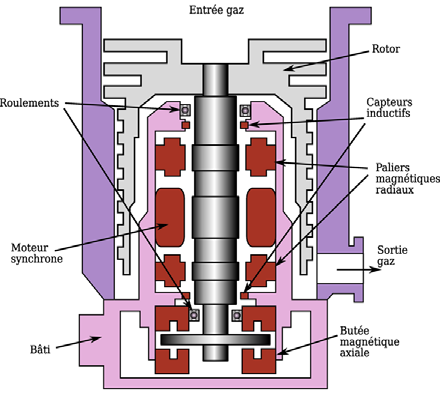
\includegraphics[width=\linewidth]{fig_05}
%\textit{}
\end{center}
\fi

\question{Comment se nomme l'action de correction obtenue avec ce terme ? }
\ifprof
\begin{corrige}
L'action de correction obtenue est de l'avance de phase. 
\end{corrige}
\else
\fi


\question{Quelle valeur doit-on donner à $\mu$ pour garantir le critère de marge de phase ? }
\ifprof
\begin{corrige}
\textbf{Cas 1 : on conserve $K_P=10$.}
 Le correcteur doit ajouter 60\degres de phase pour $\omega=\SI{6}{rad.s^{-1}}$. Il faut donc $\mu=14$.
 
 \textbf{Cas 2 : on reprend $K_P=1$.}
 Dans ce cas, on souhaite que lorsque $\omega=\SI{6}{rad.s^{-1}}$, $\varphi$ soit égal à 45\degres. Il faut donc ajouter 65\degres de phase à cette pulsation. Dans ces conditions, $\mu=20$.
 
Le critère de précision reste validé car il y a toujours les deux intégrateurs dans le correcteur. 
\end{corrige}
\else
\fi


\question{En déduire les valeurs de $T$ et de $K_P$ permettant d'assurer les critères de stabilité et de bande passante énoncés au début de partie. Le critère de précision est-il validé ?}
\ifprof
\begin{corrige}
\textbf{Dans le cas 1 :}
$\omega=\dfrac{1}{T\sqrt{\mu}}$ $ \Leftrightarrow T=\dfrac{1}{\omega\sqrt{\mu}}=\dfrac{1}{6\sqrt{14}}=\SI{0,045}{s}$.
Le gain $K_P$ déjà déterminé permet de satisfaire le cahier des charges. Il faut donc que le gain du correcteur à avance de phase soit nul à la pulsation de coupure à $\omega_{\SI{0}{dB}}$.

Il faut donc que $\dfrac{1}{2}\left( 20\log\left( \mu K_P'\right) + 20\log K_P'  \right)=0 $ 
$\Rightarrow \log\left( \mu K_P'^2\right)  =0$
$\Rightarrow  \mu K_P'^2 =1$
$\Rightarrow   K_P' =\sqrt{1/\mu}=0,267$.

\textbf{Dans le cas 2 :}
$\omega=\dfrac{1}{T\sqrt{\mu}}$ $ \Leftrightarrow T=\dfrac{1}{\omega\sqrt{\mu}}=\dfrac{1}{6\sqrt{20}}=\SI{0,037}{s}$.

Actuellement, le gain est de \SI{-20}{dB} pour $\omega=\SI{6}{rad.s^{-1}}$. Il faut donc augmenter le gain de \SI{20}{dB} pour la pulsation $\dfrac{1}{T\sqrt{u}}$. Ceci revient donc à résoudre 
$20\log K_p + \dfrac{1}{2}\left( 20\log \mu K_p  - 20\log K_p \right) = 20$
$\Rightarrow \log K_p +  \log \sqrt{\mu}= 1$
$\Rightarrow  K_p \sqrt{\mu}= 10$
$\Rightarrow  K_p = 10/\sqrt{20}=2,6$.

\textbf{Remarque : } dans le cas 1 le gain du correcteur est $K_P\times K_P' = 2,6$. Dans le cas 2  $K_p=2,6$. 

\end{corrige}
\else
\fi

\subsection*{Validation des performances}

\begin{obj}
II s'agit dans cette dernière partie de vérifier les performances globales de la boucle d'asservissement.
\end{obj}
\ifprof
\else
On donne le résultat d'une simulation du système complet piloté à l'aide du correcteur précédemment dimensionné pour une vitesse d'impact de $\SI{4}{m.s^{-1}}$.
\fi

\question{En analysant cette courbe, conclure quant à la validité du cahier des charges.}
\ifprof
\begin{corrige}
Pour une vitesse d'impact de $\SI{4}{m.s^{-1}}$ l'accélération reste bien inférieure à $\SI{3}{rad.s^{-2}}$.
\end{corrige}
\else
\fi

\ifprof
\else
\begin{marginfigure}
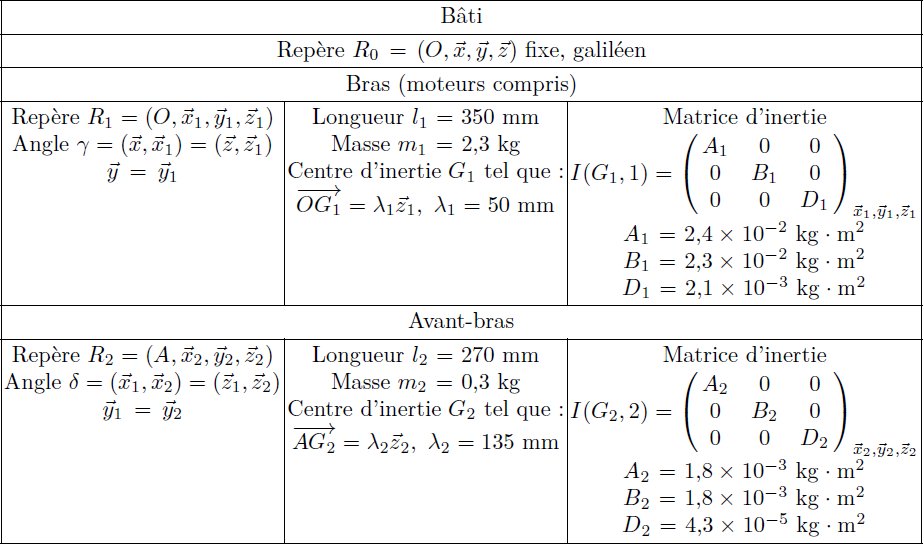
\includegraphics[width=\linewidth]{fig_06}
%\textit{}
\end{marginfigure}

\fi



\ifprof
\else
\ifcolle
\else
\marginnote{
\begin{solution}
\begin{enumerate}
\item $H_F(p)= \dfrac{K_Z p}{ 1+\left(\dfrac{2\xi_Z}{\omega_Z}+\lambda_a K_Z\right)p+\dfrac{p^2}{\omega_Z^2} }$.
\item $H_{\text{BONC}}(p) = \dfrac{K_Z p}{ 1+\left(\dfrac{2\xi_Z}{\omega_Z}+\lambda_a K_Z\right)p+\dfrac{p^2}{\omega_Z^2} } \cdot \dfrac{K_S}{1+T_Sp} $.
\item $\omega_Z= \SI{5,5}{rad.s^{-1}}$ et $K_Z=5\times 10^{-6}$.
\item 2.
\item 
\end{enumerate}
\end{solution}}
\fi
\fi

